\documentclass[11pt,a4paper]{report}

\usepackage{amssymb,amsmath,epsfig,float,subfig,hyperref,multicol}

\usepackage{xcolor}

\definecolor{SCSUred}{HTML}{CD1041}

\hypersetup{colorlinks=true,linkcolor=SCSUred,urlcolor=SCSUred}

\usepackage{enumerate}
\usepackage{tikz}
\usetikzlibrary{arrows}
\usetikzlibrary{patterns}
\usetikzlibrary{decorations}
%%\usetikzlibrary{intersections}
\usetikzlibrary{matrix}
\usetikzlibrary{snakes}
\usetikzlibrary{calc}
\usetikzlibrary{backgrounds}

\definecolor{linecolor}{HTML}{0074C8}
\definecolor{linecolor2}{HTML}{C80200}

\newcommand{\imagebullet}[1]{\includegraphics[width=0.5cm]{#1}}

\pagestyle{empty}
\setlength{\textwidth}{7in}
\setlength{\textheight}{10in}
\setlength{\oddsidemargin}{-25pt}
\setlength{\evensidemargin}{-25pt}
\setlength{\topmargin}{-50pt}

\usepackage[english]{babel}
\usepackage[utf8]{inputenc}
\usepackage{fancyhdr}
 
%%\pagestyle{fancy}
\renewcommand{\headrulewidth}{0pt}
%%\fancyhf{}
%%\rhead{Share\LaTeX}
%%\lhead{Guides and tutorials}
%%\cfoot{OVER}

\newcommand{\DueA}{Monday, October 7}
\newcommand{\DueB}{Tuesday, October 8}
\newcommand{\DueC}{Tuesday, October 15}
%%\newcommand{\DueD}{Tuesday, October 8}

\begin{document}

\begin{figure}[ht]
\begin{flushright}
	\includegraphics[width=2.0in]{U_PriHorz_WhtLtBG.jpg}
	\end{flushright}
\end{figure}

\vspace{-12mm}

\begin{flushleft}
\Large\bf \href{https://activecalculus.org/single/sec-2-5-chain.html}{2.5 - The Chain Rule}\rm
%%Daily Preparation - \DueA \rm
\end{flushleft}


\vspace{8pt}

\noindent {\Large\bf{Overview}} \\
We have come a long way in just over a week's time: from the initial basic rules for power and exponential functions, to the structure rules given by the sum and constant multiple rules, then the basic rules for the sine and cosine functions, followed by the more complicated structure rules given by the product and quotient rules. With those rules in hand, we have found derivatives for the remaining trigonometric functions, and we are now ready to deal with one more way that functions can be combined: composite functions, also known as chains of functions. The derivative rule which helps us deal with these is called the {\it{Chain Rule}}.

%%This section covers the following concept: Linearization of a function.



\vspace{16pt}

%%\pagebreak

\noindent {\Large\bf{To prepare for class}} \\
Complete all actions listed below.  Respond to the questions highlighted with {\color{SCSUred}{\boxed{Submit}}}.  %% by the start of class on {\bf{\DueA}}.  A single .pdf should be uploaded to D2L Brightspace.
\begin{itemize} \itemsep -2pt % Reduce space between items

\item {\bf{Read}} motivating questions and the introduction to \href{https://activecalculus.org/single/sec-2-5-chain.html}{section 2.5} (up until Preview Activity 2.5.1).
\item[{\color{SCSUred} \boxed{Submit}}] {\bf{Do}} \href{https://activecalculus.org/single/sec-2-5-chain.html#vLx}{Preview Activity 2.5.1}.

\item[\imagebullet{CopilotLogo.jpg} {\color{SCSUred} \boxed{Submit}}] Ask {\bf{Copilot}} ``Explain, in the simplest of terms, why the chain rule formula in calculus is the way it is.  Be sure that I see the chain of variables that is involved.  Maybe focus on a food chain for me."  Submit two sentences summarizing the idea returned by the AI.  

\item {\bf{Do}} these problems.
\begin{enumerate}
\setcounter{enumi}{0}
\item Imagine we are moving straight upward in a hot air balloon.  Let $y$ be our distance from the ground.  The temperature, $H$, is changing as a function of altitude, so $H = f(y)$.  In fact, it decreases at a rate of $16^{\circ} F$ per mile.  Meanwhile, our balloon is climbing at a rate of 2 miles per hour (mph).  How much does our temperature change during our first 15 minutes?
  
\item In the previous problem, temperature is a function of height, $H = f(y)$, and height is a function of time, $y=g(t)$.  So, we can think of temperature as a composite function of time, $H=f(g(t))$ ,with $f$ as the outside function and $g$ as the inside function.  For the functions below, identify a composite function $C(t)$ by describing an outside function $f$ and an inside function $g$.  
\begin{enumerate}
\item $C(t) = (t^2+1)^{100}$
\item $C(t) = \sqrt{3t^2 + 5t+2}$
\item The length $C$ (in micrometers) of steel depends on the air temperature (in $^{\circ}C$), and the temperature depends on time, $t$, measured in hours.  The length of a steel bridge increases by 0.2 micrometers for every degree increase in temperature (and is 1 micrometer at temperature of $0^{\circ}C$).  The temperature is increasing at $3^{\circ}C$ per hour and is $4^{\circ}C$ at time $t=0$ hours.  
\end{enumerate}
%%\item Suppose that for an increase of 100 mosquitoes in the population, the number of little brown bats increases by 1.  Suppose also that for an increase of 10 little brown bats in the population, the number of snakes increases by 1.  By how much does the snake population change with an increase of 5,000 mosquitoes in the population?
\end{enumerate} 

\item {\bf{Read}} \href{https://activecalculus.org/single/sec-2-5-chain.html#Utl}{section 2.5.1}.

\item {\bf{Watch}} video \href{https://www.youtube.com/watch?v=HxVn6kRD5NM&feature=emb_title}{Quick Review - The Chain Rule (2:20)}.  

\item[{\color{SCSUred} \boxed{Submit}}] {\bf{Do}} the following construction in \href{https://www.geogebra.org/classic}{\it{GeoGebra}} that may help convince you of the accuracy of the chain rule.  Submit screenshots and answers to the questions posed as needed.
\begin{itemize}
\item In \href{https://www.geogebra.org/classic}{\it{GeoGebra}}, type {\tt{sqrt(x)}} in the input box.  The function $f(x) = \sqrt{x}$ will be defined and graphed.  
\item In the next input box, type {\tt{2*x+3}}.  The function $g(x) = 2x+3$ will be defined and graphed.  
\item In the third input box, we define the composite function $h(x)=f(g(x))$.  To do so, simply type {\tt{f(g(x))}}.  {\it{GeoGebra}} should output $\sqrt{2x+3}$.  
\item We will now pick a point on the graph of $h$ to measure the slope (i.e. the derivative of $h$).  In the next input box, type {\tt{A = (3, h(3))}}.  {\it{GeoGebra}} will plot the point $A$ at $(3,3)$.  On the fourth button (see below), choose the {\tt{Tangents}} option.  Then, click on point {\tt{A}} on your graph followed by clicking on the graph (of $h$) itself.  This will produce a tangent line to your function $h$ at $(3,3)$.  It will name this tangent line and an expression for it will appear in the next input box.  From this tangent line equation, the value of $h'(3)$ should be obvious.  What is it?  
\begin{figure}[H]
\begin{center}
	\includegraphics[width=2.0in]{TangentsGeoGebra.jpg}
	\end{center}
\end{figure}  
\item Now we verify that $h'(3) = f'(g(3))\cdot g'(3)$.  To that end, in the next input box type {\tt{g'(3)}}.  {\it{GeoGebra}} should compute this value and name it $a$.  Does the value returned make sense?  
\item Repeat this process to compute $f'(g(3))$ by typing {\tt{f'(g(3))}} in the next input box.  {\it{GeoGebra}} will compute this value and name it $b$.  In the final input box, type {\tt{a * b}}.  This should be the same as $h'(3)$ (found earlier).  Is it?  
\end{itemize}  



\item {\bf{Watch}} video \href{https://www.youtube.com/watch?v=QDc1UmLWhug&list=PL9bIjQJDwfGuXQHuS5Jkmum_CFILoCZX-&index=41}{Examples of the Chain Rule - Polynomials (4:32)}.

%%\item {\bf{Do}} Activity 2.5.2.  



\end{itemize}









\vspace{16pt}

\noindent {\Large\bf{After class}}\\
Solidifying the concepts discussed in class through practice is necessary to build your skills. 

%%\noindent {\large\bf{After \DueA}}
\begin{itemize}\itemsep -2pt % Reduce space between items
\item {\bf{Read}} \href{https://activecalculus.org/single/sec-2-5-chain.html#AAu}{section 2.5.2}.



\item {\bf{Watch}} video \href{https://www.youtube.com/watch?v=ysp96e3Z-nw&list=PL9bIjQJDwfGuXQHuS5Jkmum_CFILoCZX-&index=41}{Examples of the Chain Rule - Radicals (7:19)}.  
  
\item {\bf{Watch}} video \href{https://www.youtube.com/watch?v=4y39u0DmrPY&list=PL9bIjQJDwfGuXQHuS5Jkmum_CFILoCZX-&index=42}{Examples of the Chain Rule - Trigonometric Functions (5:14)}. 

\item {\bf{Watch}} video \href{https://www.youtube.com/watch?v=zexX6t_zbCg&list=PL9bIjQJDwfGuXQHuS5Jkmum_CFILoCZX-&index=43}{Examples of the Chain Rule - Exponential Functions (6:00)}. 
 

\item {\bf{Do}}  \href{https://activecalculus.org/single/sec-2-5-chain.html#dJG}{Exercises 1-3 in section 2.5}.

%%\item {\bf{Do}} Activity 2.5.3.

\item {\bf{Watch}} video \href{https://www.youtube.com/watch?v=pwm50foAx6A&list=PL9bIjQJDwfGuXQHuS5Jkmum_CFILoCZX-&index=45}{Chain Rule Examples - Graphs Only (5:37)}. 
 
\item {\bf{Do}} this problem.
\begin{enumerate}
\setcounter{enumi}{2}
\item The graph of $f(x)$ is given below.  It is known that $f'(0)=-1$, $f'(1) = \frac{3}{4}$, $f'(2)=1$, and $f'(4) = -3$. Define $h(x) = f(x^2)$.  
 \begin{figure}[H]
\flushright
{
  \begin{tikzpicture}[thick,scale=1] [domain=-1:4.5]
\draw[step=1cm,color=gray!50] (-1,-2) grid (5,2);
   \draw [black!80,line width=0.3pt,-latex] (0,0) -- (5,0) node [below] at (4.75,0) {$x$};
   \draw [black!80,line width=0.3pt,-latex] (0,0) -- (-1,0);
   \draw [black!80,line width=0.3pt,-latex] (0,0) -- (0,2) node [right] at (0,1.75) {$y$};
   \draw [black!80,line width=0.3pt,-latex] (0,0) -- (0,-2);
\draw[color=blue, line width=1.5pt,domain=-0.85:4.5]   plot[smooth] (\x,{-0.25*\x*\x*\x+1.25*\x*\x-\x}) node [right] at (3.5, 1.2) {$f(x)$};
%%\draw[color=blue, line width=1pt,domain=-1:1]   plot (\x,{2*\x+3});
%%\draw[color=blue, line width=1pt,domain=1:5]   plot (\x,{-0.5*\x+5.5});
%%  node[above] at (2,1) {$f(3,y)$};
\foreach \x/\xtext in {1/1, 2/2, 3/3,4/4}
    \draw[shift={(\x,0)}] (0pt,3pt) -- (0pt,-3pt) node[below] {$\xtext$};
\foreach \y/\ytext in {-1/-1, 1/1}
    \draw[shift={(0,\y)}] (-2pt,0pt) -- (2pt,0pt) node[left] {$\ytext$};
\end{tikzpicture}}  
\end{figure}

\vspace{-50mm}
\begin{enumerate}
\item Compute $h(-1)$, $h(0)$, $h(1)$, $h(\sqrt{2})$, and $h(2)$. 
\vspace{35mm} 
\item Compute $h'(0)$, $h'(-2)$, and $h'(2)$.  
\vspace{5mm}
%%\vspace{25mm} 
\item The graph of $h(x)$ is shown.  \\
Do the above values make sense? 
\vspace{-10mm} 
 \begin{figure}[H]
\flushright
{
  \begin{tikzpicture}[thick,scale=0.85] [domain=-2.25:2.25]
\draw[step=1cm,color=gray!50] (-3,-2.5) grid (3,2);
   \draw [black!80,line width=0.3pt,-latex] (0,0) -- (3,0) node [below] at (2.75,0) {$x$};
   \draw [black!80,line width=0.3pt,-latex] (0,0) -- (-3,0);
   \draw [black!80,line width=0.3pt,-latex] (0,0) -- (0,2) node [right] at (0,1.75) {$y$};
   \draw [black!80,line width=0.3pt,-latex] (0,0) -- (0,-2.5);
\draw[color=blue, line width=1.5pt,domain=-2.15:2.15]   plot[smooth] (\x,{-0.25*\x*\x*(\x*\x-1)*(\x*\x-4)}) node [right] at (2,1.2) {$h(x)$};
%%\draw[color=blue, line width=1pt,domain=-1:1]   plot (\x,{2*\x+3});
%%\draw[color=blue, line width=1pt,domain=1:5]   plot (\x,{-0.5*\x+5.5});
%%  node[above] at (2,1) {$f(3,y)$};
\foreach \x/\xtext in {-2/-2, -1/-1, 1/1, 2/2}
    \draw[shift={(\x,0)}] (0pt,3pt) -- (0pt,-3pt) node[below] {$\xtext$};
\foreach \y/\ytext in {-2/-2, -1/-1, 1/1}
    \draw[shift={(0,\y)}] (-2pt,0pt) -- (2pt,0pt) node[left] {$\ytext$};
\end{tikzpicture}}  
\end{figure}
\end{enumerate}
\end{enumerate}



%%\end{itemize}

%%\pagebreak

%%\noindent {\large\bf{After \DueB}}
%%\begin{itemize}\itemsep -2pt % Reduce space between items
\item {\bf{Watch}} video \href{https://www.youtube.com/watch?v=1B06Pk3W6Pc&list=PL9bIjQJDwfGuXQHuS5Jkmum_CFILoCZX-&index=44}{Chain Rule Examples - Mixing Rules (10:29)}. 

\item[\imagebullet{CopilotLogo.jpg}] Prompt {\bf{Copilot}} ``Generate an example of a problem using a table where I would be asked to calculate the derivative of a composition of two functions using the chain rule.  Be sure to also generate a solution for me."  Does the AI return a correct solution?  


\item {\bf{Read}} \href{https://activecalculus.org/single/sec-2-5-chain.html#gHD}{section 2.5.3}.

\item {\bf{Do}}  \href{https://activecalculus.org/single/sec-2-5-chain.html#xJB}{Exercises 4-11 in section 2.5}. 
%%\item {\bf{Do}} Activity 2.5.4.


%%\item {\bf{Do}}  \href{https://activecalculus.org/single/sec-2-5-chain.html#Wml}{Exercises 8-9 in section 2.5}.

%%\end{itemize}

%%\noindent {\large\bf{After \DueD}}
%%\begin{itemize}\itemsep -2pt % Reduce space between items
%%\item {\bf{Do}}  \href{https://activecalculus.org/single/sec-2-5-chain.html#iAD}{Exercises 10-11 in section 2.5}.
\item {\bf{Start working}} on the \href{https://www.myopenmath.com/index.php}{MOMwork} (MyOpenMath) assignment for this section.  %%This will be due on \DueC.   
\end{itemize}

%%\pagebreak

\vspace{16pt}

\noindent {\Huge\bf{Extra Prep}}

\vspace{16pt}

\noindent {\Large\bf{Basic learning objectives}}\\
These are the tasks you should be able to perform with reasonable
fluency when you arrive at our next class meeting. Important new
vocabulary words are indicated {\it{in italics}}.  Check each box when you feel confident you have a firm grasp on that objective.

\begin{itemize} \itemsep -2pt % Reduce space between items
\renewcommand{\labelitemi}{\scriptsize$\square$}
\item State, from memory, all of the basic function and structure rules noted in the {\it{Overview}} above.
\item Identify the ``inner" and `outer" function in a composite function of the form $C(x) = f(g(x))$, such as in $C(x) = e^{x^2+1}$ or $C(x) = \sqrt{\cos x + 4}$.  
\item State the Chain Rule:$\displaystyle \frac{d}{dx} f(g(x)) = \hdots$
\end{itemize}

\vspace{16pt}

\noindent {\Large\bf{Advanced learning objectives}}\\
In addition to mastering the basic objectives, here are the tasks you should be able to perform after class, with practice:
\begin{itemize} \itemsep -2pt % Reduce space between items
\renewcommand{\labelitemi}{\scriptsize$\square$}
\item Apply the Chain Rule to basic examples.
\item Differentiate functions that require the application of multiple rules. For instance, compute the derivative of $\displaystyle g(x) = \frac{\sin^2(x) \cdot e^{x-5}}{\sqrt{x^2+1}}$.  

\end{itemize}

\vspace{16pt}

\noindent {\Large\bf{Need More Help?}}

\begin{itemize}\itemsep -2pt % Reduce space between items
\item {\bf{Watch}} video \href{https://www.youtube.com/watch?v=Xt5a59Sc7Aw&feature=youtu.be}{Chain Rule - Student Problem Solving (5:53)}.  

\item  {\bf{Watch}} video \href{https://www.youtube.com/watch?v=g8mWdHea0ao&feature=youtu.be}{Average Rates of Change of Composite Functions (5:04)}.

\item {\bf{Watch}} video \href{https://www.youtube.com/watch?v=VdsJVaTI7HY&feature=youtu.be}{How to use the Chain Rule (5:27)}.
\item {\bf{Watch}} video \href{https://www.youtube.com/watch?v=iezUUzupaSk&feature=youtu.be}{Why Chain Rule Works (5:14)}.
\item  {\bf{Explore}} the following applet (especially if you are mechanical engineering major(?): \href{https://webspace.ship.edu/msrenault/GeoGebraCalculus/derivative_intuitive_chain_rule.html}{The intuitive notion of the chain rule}.  At first glance, the moving belts will make the chain rule jump out at you! 
\item  {\bf{Watch}} video \href{https://www.youtube.com/watch?v=6oMt3f2q4Ik&feature=emb_title}{Chain rule $u$-notation (9:27)}.  [If you would like more examples with the chain rule...one really can't get enough - the chain rule is a crucial topic to your success.]

\item  {\bf{Watch}} video \href{https://www.youtube.com/watch?v=f56aAclfVEA&feature=emb_title}{Combining the Chain Rule with the Product or Quotient Rule (4:13)}.

\item {\bf{Watch}} video \href{https://www.youtube.com/watch?time_continue=23&v=l0b-bhpBy44&feature=emb_title}{Applied Example (tides) involving the differentiation of a trigonometric function (10:35)}.

\item {\bf{Do}} these problems.
\begin{enumerate}
\setcounter{enumi}{3}

\item Consider the functions $f$ and $g$ given by the graph.  Define $h(x) = f(g(x))$.  
 \begin{figure}[H]
\flushright
{
  \begin{tikzpicture}[thick,scale=0.75] [domain=-2:10]
\draw[step=1cm,color=gray!50] (-2,-2) grid (10,6);
   \draw [black!80,line width=0.3pt,-latex] (0,0) -- (10.5,0) node [above] at (10.25,0) {$x$};
   \draw [black!80,line width=0.3pt,-latex] (0,0) -- (-2,0);
   \draw [black!80,line width=0.3pt,-latex] (0,0) -- (0,6.5) node [right] at (0,6.25) {$y$};
   \draw [black!80,line width=0.3pt,-latex] (0,0) -- (0,-2);
\draw[color=blue, line width=1pt,domain=-0.66:2]   plot[smooth] (\x,{3*\x});
\draw[color=blue, line width=1pt,domain=2:10]   plot[smooth] (\x,{-0.75*\x+7.5}) node [right] at (9,1) {$g$};
\draw[color=blue, line width=1.5pt,domain=-2:4.01]   plot[smooth] (\x,{0.333*\x*\x - 0.667*\x + 1.333});
\draw[color=blue, line width=1.5pt,domain=4:10]   plot[smooth] (\x,{0.33*\x+2.667}) node [right] at (7,4.5) {$f$};
\foreach \x/\xtext in {-1/-1, 1/1, 2/2, 3/3, 4/4, 5/5, 6/6, 7/7, 8/8, 9/9}
    \draw[shift={(\x,0)}] (0pt,3pt) -- (0pt,-3pt) node[below] {$\xtext$};
\foreach \y/\ytext in { -1/-1, 1/1, 2/2, 3/3, 4/4, 5/5}
    \draw[shift={(0,\y)}] (-2pt,0pt) -- (2pt,0pt) node[left] {$\ytext$};
\end{tikzpicture}}  
\end{figure}

\vspace{-75mm}
\begin{enumerate}
\item Compute $h'(1)$.
\vspace{15mm}
\item Compute $h'(0)$.
\vspace{15mm}
\item Does $h'(2)$ exist? \\ If so, compute its value.  \\ If not, why not?
\vspace{15mm}
\end{enumerate}



\item Use information from the graphs of $f(x)$ and $g(x)$ and the tangent lines shown to calculate $m'(2)$ if $m(x) = g(f(x))$.
%%\begin{enumerate}
%%\item $h'(2)$ if $h(x) = \tan^{-1}(f(x))$
%%\vspace{40mm}
%%\item $k'(2)$ if $\displaystyle k(x) = \frac{f(x)}{g(x)}$
%%\vspace{40mm}
%%\item 
%%\end{enumerate}

%%\vspace{-30mm}
 \begin{figure}[H]
\centering
{
  \begin{tikzpicture}[thick,scale=0.75] [domain=-1:10]

\draw[color=blue, line width=1pt,domain=1:7]   plot (\x,{0.1*(\x-2)*(\x-5)*(\x-5)+3}) node [above] at (5,3) {$f(x)$};
\draw[color=black, line width=1pt,domain=1.25:4.2]   plot (\x,{0.9*\x+1.2});
\fill [black] (2,3) circle (4pt) node [left] at (2,3) {$(2,3)$};
\fill [black] (4,4.8) circle (4pt) node [left] at (4,4.8) {$(4,4.8)$};

\end{tikzpicture}}  
\end{figure}

\vspace{-35mm}
 \begin{figure}[H]
\flushright
{
  \begin{tikzpicture}[thick,scale=0.75] 

\draw[color=blue, line width=1pt,domain=-1:2]   plot (\x,{5-\x*\x}) node [above] at (-1.5,4) {$g(x)$};
\draw[color=black, line width=1pt,domain=0.7:2.1]   plot (\x,{-2*\x+6});
\draw[color=black, line width=1pt,domain=-2.25:1]   plot (\x,{5});
\fill [black] (1,4) circle (4pt) node [right] at (1,4) {$(3,4)$};
\fill [black] (1.5,3) circle (4pt) node [right] at (1.5,3) {$(3.5,3)$};
\fill [black] (0,5) circle (4pt) node [above] at (0,5) {$(2,5)$};
\fill [black] (-2,5) circle (4pt) node [above] at (-2,5) {$(0,5)$};

\end{tikzpicture}}  
\end{figure}

%%\end{enumerate}

%%\item {\bf{Do}} these problems.
%%\begin{enumerate}
%%\setcounter{enumi}{5}
\item If $g(x) = \sqrt{f(x)}$, where the graph of $f$ \\
and a tangent line is shown, evaluate $g'(3)$.
\vspace{-15mm}
 \begin{figure}[H]
\flushright
{
  \begin{tikzpicture}[thick,scale=0.9] [domain=-1:7]
\draw[step=1cm,color=gray!50] (-1,-1) grid (7,6);
   \draw [black!80,line width=0.3pt,-latex] (0,0) -- (7.5,0) node [above] at (7.25,0) {$x$};
   \draw [black!80,line width=0.3pt,-latex] (0,0) -- (-1,0);
   \draw [black!80,line width=0.3pt,-latex] (0,0) -- (0,6.5) node [right] at (0,6.25) {$y$};
   \draw [black!80,line width=0.3pt,-latex] (0,0) -- (0,-1);
\draw[color=blue, line width=1.5pt,domain=-0:6]   plot[smooth] (\x,{-0.6667*\x+4});
%%\draw[color=blue, line width=1pt,domain=-2:4.01]   plot[smooth] (\x,{0.333*\x*\x - 0.667*\x + 1.333});
\draw[color=red, line width=1.5pt,domain=-1:7]   plot[smooth] (\x,{-sin(\x*45-180)+1.25}) node [right] at (6.5,0.75) {$f$};
\fill [black] (3,2) circle (3pt); %%node [right] at (1,4) {$(3,2$};
\foreach \x/\xtext in { 1/1, 2/2, 3/3, 4/4, 5/5, 6/6}
    \draw[shift={(\x,0)}] (0pt,3pt) -- (0pt,-3pt) node[below] {$\xtext$};
\foreach \y/\ytext in { 1/1, 2/2, 3/3, 4/4, 5/5}
    \draw[shift={(0,\y)}] (-2pt,0pt) -- (2pt,0pt) node[left] {$\ytext$};
\end{tikzpicture}}    
\end{figure}

\item For each of the following functions of $x$, write the equation for the derivative function.  Please do us both a favor and don't simplify the answers.  
\begin{enumerate}
\item $y = \sin 3x$ 
%%\vspace{25mm}
\item $w = (\sin 3x)^3$
%%\vspace{35mm}
\item $u = (\sin 3x)^3 + 5x$
%%\vspace{35mm}
\item $v = \left[ (\sin 3x)^3 + 5x \right]^2$
%%\vspace{35mm}
\item $\displaystyle k(x) = x + \frac{1}{x}$
%%\vspace{25mm}
\item $\displaystyle l(x) = \sqrt{x + \frac{1}{x}}$
%%\vspace{25mm}
\item $\displaystyle m(x) = \left[ (\sin 3x)^3 + 5x \right]^2 \cdot \sqrt{x + \frac{1}{x}}$
%%\vspace{25mm}
\end{enumerate}

\item Differentiate $\displaystyle y = \sqrt{1+e^{\sqrt{3+x^2}}}$. 

\end{enumerate}

\end{itemize}
 
\vspace{16pt}

\noindent {\Large\bf{Selected Answers}}
\begin{enumerate}
\setcounter{enumi}{0}

\item $\frac{dH}{dy} = -16\frac{^{\circ}F}{mi}$ and $\frac{dy}{dt}= 2 \frac{mi}{hr}$ means that $\frac{dH}{dt} = \frac{dH}{dy} \cdot \frac{dy}{dt} = (-16)(2) = -32 \frac{^{\circ}F}{hr}$.  In 15 minutes, $H$ changes $1/4$ of this or $-8^{\circ}F$ (a decrease of 8 degrees Fahrenheit).  

\item 
\begin{enumerate}
\item $g(t) = t^2+1$ and $f(t) = t^100$, though answers may vary.
\item $g(t) =3t^2 + 5t + 2$ and $f(t) = \sqrt{t}$, though answers may vary.
\item $g(t) =3t+4$ and $f(t) = 0.2t+1$, though answers may vary. 
\end{enumerate}

\item 
\begin{enumerate}
\item $h(-1)=f(1)=0$, $h(0)=f(0)=0$, $h(1)=f(1)=0$, $h(\sqrt{2})=f(2)=1$, $h(2)=f(4)=0$.
\item $h'(x)=f'(x^2)\cdot 2x$ so that $h'(0)=f'(0)\cdot (2)(0)=0$, $h'(-2) = f'(4)\cdot (2)(-2) = 12$, and $h'(2)=f'(4)\cdot (2)(2) = -12$.
\item Yes
\end{enumerate}

\item 
\begin{enumerate}
\item $h'(x) = f'(g(x))g'(x)$ so that $h'(1) = f'(g(1))g'(1) = f'(3)g'(1) = f'(3)\cdot 3 = \frac{2}{3}(2)(3) = 4$; Note that on $(-2,4)$, the function $f(x)$ can be found to be $f(x) = \frac{1}{3}(x-1)^2 + 1$ by noting it has vertex at $(1,1)$ and the point $(4,4)$ determines $c$ in $f(x) = c(x-1)^2 + 1$.  
\item $h'(0)=f'(g(0))g'(0)=f'(0)\cdot 3 = \frac{2}{3} \cdot 3 = 2$.
\item $h'(2)$ does not exist since $g'(2)$ does not exist.  $h$ is not `smooth` at $x=2$. 
\end{enumerate}

\item $m'(x) = g'(f(x))f'(x)$ so that $m'(2) = g'(f(2)) \cdot f'(2) = g'(3) \cdot \left( \frac{4.8-3}{4-2} \right) = \left( \frac{4-3}{3-3.5} \right) (0.9) = -2(0.9) = -1.8$.  

\item $\displaystyle g'(x) = \frac{1}{2}f(x)^{-1/2} \cdot f'(x) = \frac{1}{2\sqrt{f(x)}} \cdot f'(x)$.  Thus, $\displaystyle g'(3) = \frac{1}{2\sqrt{f(3)}} \cdot f'(3) = \frac{1}{2\sqrt{2}} \cdot \left( \frac{2-4}{3-0} \right) = -\frac{1}{3\sqrt{2}}$.  

\item 
\begin{enumerate}
\item If $z=3x$, then $\displaystyle \frac{dy}{dx} = \frac{dy}{dz} \cdot \frac{dz}{dx} = \cos z \cdot 3 = 3 \cos(3x)$.
\item Here, $w= y^3$ so that $\displaystyle \frac{dw}{dx} = \frac{dw}{dy} \frac{dy}{dz} \frac{dz}{dx} = 3y^2 \cdot \cos z \cdot 3 = 9 \sin^2 (3x) \cos (3x)$.
\item Here $u = w^3 + 5x$ so that $\displaystyle \frac{du}{dx} = \frac{du}{dw} \frac{dw}{dx} + 5 = 3w^2 \cdot  9 \sin^2 (3x) \cos (3x) + 5 = 27 \sin^6 (3x) \cdot \sin^2 (3x) \cos (3x) + 5 = 27 \sin^8 (3x) \cos (3x) + 5$.  
\item Here $v = u^2$ so that $\displaystyle \frac{dv}{dx} = \frac{dv}{du} \frac{du}{dx} = 2u \frac{du}{dx} = 2 \left( \sin^3 (3x) + 5x \right) \left( 27 \sin^8 (3x) \cos (3x) + 5 \right)$.
\item $\displaystyle \frac{dk}{dx} = 1 -\frac{1}{x^2}$.  
\item Here, $l = \sqrt{k}$ so that $\displaystyle \frac{dl}{dx} = \frac{dl}{dk}\frac{dk}{dx} = \frac{1}{2} k^{-1/2} \left( 1-\frac{1}{x^2} \right) = \frac{1}{2\sqrt{x+\frac{1}{x}}} \left(1 - \frac{1}{x^2} \right)$.  
\item Here $m(x) = v(x) \cdot l(x)$ so that by the product rule $\displaystyle \frac{dm}{dx} = \frac{dv}{dx} l(x) + v(x) \frac{dl}{dx} $ = $$2 \left( \sin^3 (3x) + 5x \right)(27 \sin^8 (3x) \cos (3x) + 5 ) \sqrt{x + \frac{1}{x}} + \left( \sin^3 (3x) + 5x \right)^2 \cdot  \frac{1}{2\sqrt{x+\frac{1}{x}}} \left(1 - \frac{1}{x^2} \right).$$
\end{enumerate}

\item $\displaystyle \frac{dy}{dx} = \frac{1}{2} \left( 1+e^{\sqrt{3+x^2}} \right)^{-1/2} \cdot e^{\sqrt{3+x^2}} \cdot \frac{1}{2} (3+x^2)^{-1/2} \cdot 2x$.  

\end{enumerate}

\end{document}

